\documentclass{article}
%
\usepackage{mathbbol}

\usepackage{ctex}
\usepackage{geometry}
\usepackage[dvipsnames, svgnames, x11names]{xcolor}
\usepackage[mathscr]{euscript}
\usepackage{tikz}
\usepackage{xstring}
%

\usetikzlibrary{decorations.pathreplacing}
\usetikzlibrary{positioning, arrows.meta, automata}
%
%
\begin{document}
%
\begin{center}
  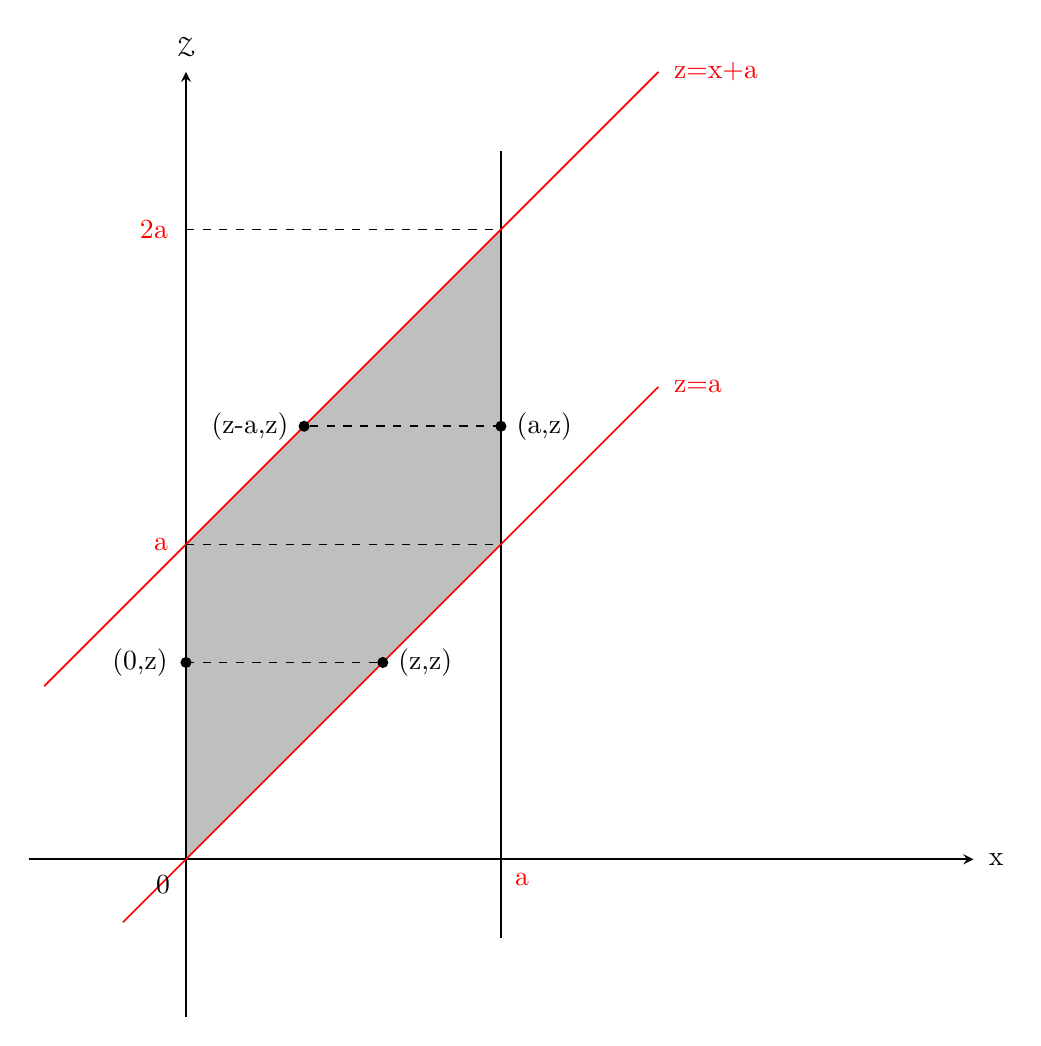
\begin{tikzpicture}[->,>=stealth,node distance=2cm,semithick,initial text=,]
    \fill[lightgray] (0,0)--(0,4)--(4,8)--(4,4)--cycle;

    \draw[->] (-2,0) to (10,0);
    \draw[->] (0,-2) to (0,10);
    \draw[-] (0,10) node [above = 2pt]{$\mathscr{Z}$};
    \draw[-] (10,0) node [right = 2pt]{x};

    \draw[-] (4,-1) to (4, 9);

    \draw[-, color=red] (-0.8,-0.8) to (6,6);
    \draw[-] (6,6) node [right=2pt ,red]{z=a};
    \draw[-] (6,10) node [right=2pt ,red]{z=x+a};
    
    \draw[-, color=red] (-1.8,2.2) to (6,10);
    \draw[-] (0,4) node [left = 3pt, color=red]{a};
    \draw[-] (0,8) node [left = 3pt, color=red]{2a};
    \draw[-] (0,0) node [below left = 3pt]{0};
    \draw[-] (0,2.5) node [left = 3pt]{(0,z)};
    \fill (0,2.5) circle (2pt);

    \fill (2.5,2.5) circle (2pt) node [right=2pt]{(z,z)};
    \draw[-, dashed] (0,2.5) to (2.5,2.5);

    \fill (1.5,5.5) circle (2pt) node [left=2pt]{(z-a,z)};
    \fill (4,5.5) circle (2pt) node [right=2pt]{(a,z)};
    \draw[-, dashed] (4,5.5) to (1.5,5.5);
    \draw[-, dashed] (0,4) to (4,4);
    \draw[-, dashed] (0,8) to (4,8);

    \draw[-] (4,0) node [red, below right=2pt]{a};




  \end{tikzpicture}
  \heiti\\ 图10.2 被积函数非负的积分区域\songti
\end{center}
%
\end{document}
